\documentclass[12pt,a4paper]{article}

% ── Packages ────────────────────────────────────────────────────────────────
\usepackage[top=2.5cm, bottom=2.5cm, left=2.5cm, right=2.5cm]{geometry}
\usepackage[table,dvipsnames]{xcolor}
\usepackage{graphicx}
\usepackage{fancyhdr}
\usepackage{titlesec}
\usepackage[most,breakable]{tcolorbox}
\usepackage{booktabs}
\usepackage{tabularx}
\usepackage{array}
\usepackage{multirow}
\usepackage{colortbl}
\usepackage{enumitem}
\usepackage[hidelinks]{hyperref}
\usepackage{float}
\usepackage{caption}
\usepackage{subcaption}
\usepackage{parskip}
\usepackage{amsmath}
\usepackage{microtype}
\usepackage[T1]{fontenc}
\usepackage[utf8]{inputenc}
\usepackage{lmodern}
\usepackage{pifont}
\usepackage{textcomp}
\usepackage{mdframed}
\usepackage{setspace}

% ── Colour palette ───────────────────────────────────────────────────────────
\definecolor{Navy}{HTML}{1B3A6B}
\definecolor{Steel}{HTML}{2E75B6}
\definecolor{Teal}{HTML}{0D7377}
\definecolor{LightBg}{HTML}{F2F4F8}
\definecolor{Border}{HTML}{D0D7E4}
\definecolor{DarkText}{HTML}{1A1A1A}
\definecolor{StatusGreen}{HTML}{27AE60}
\definecolor{StatusAmber}{HTML}{E67E22}
\definecolor{StatusRed}{HTML}{C0392B}
\definecolor{HeaderBg}{HTML}{EAF1FB}
\definecolor{CoverBg}{HTML}{1B3A6B}

% ── Section styling ──────────────────────────────────────────────────────────
\titleformat{\section}
  {\Large\bfseries\color{Navy}}{}
  {0em}{}
  [\vspace{-4pt}\color{Steel}\rule{\linewidth}{1.5pt}]

\titleformat{\subsection}
  {\large\bfseries\color{Navy}}{}
  {0em}{}

\titleformat{\subsubsection}
  {\normalsize\bfseries\color{Teal}}{}
  {0em}{}

\titlespacing*{\section}{0pt}{18pt}{8pt}
\titlespacing*{\subsection}{0pt}{12pt}{4pt}
\titlespacing*{\subsubsection}{0pt}{8pt}{2pt}

% ── Header / Footer ──────────────────────────────────────────────────────────
\pagestyle{fancy}
\fancyhf{}
\renewcommand{\headrulewidth}{0pt}
\fancyhead[L]{\small\color{Navy}\textbf{InfraCore Systems LLP}}
\fancyhead[R]{\small\color{Navy}PoC Progress Report --- Precision Guidance System}
\fancyfoot[C]{\small\color{Border}\thepage}
\fancyfoot[R]{\footnotesize\color{Border}Confidential}

% ── Spacing ──────────────────────────────────────────────────────────────────
\setlength{\parindent}{0pt}
\setlength{\parskip}{6pt}

% ── tcolorbox styles ─────────────────────────────────────────────────────────
\tcbuselibrary{skins,breakable}

\newtcolorbox{reportbox}[2][]{
  enhanced, breakable,
  colback=LightBg, colframe=Steel,
  fonttitle=\bfseries\color{white}, coltitle=white,
  colbacktitle=Navy,
  attach boxed title to top left={yshift=-2mm, xshift=6mm},
  boxed title style={colframe=Navy, sharp corners},
  sharp corners, boxrule=0.5pt,
  title={#2}, #1
}

\newtcolorbox{feedbackbox}{
  enhanced, breakable,
  colback=StatusAmber!8, colframe=StatusAmber,
  fonttitle=\bfseries\color{white}, coltitle=white,
  colbacktitle=StatusAmber,
  attach boxed title to top left={yshift=-2mm, xshift=6mm},
  boxed title style={colframe=StatusAmber, sharp corners},
  sharp corners, boxrule=0.5pt,
  title={Evaluator Feedback}
}

% ── Status marks ─────────────────────────────────────────────────────────────
\newcommand{\chk}{\textcolor{StatusGreen}{\ding{52}}}
\newcommand{\prt}{\textcolor{StatusAmber}{\ding{119}}}
\newcommand{\pnd}{\textcolor{StatusRed}{\ding{54}}}

% ── Table column types ───────────────────────────────────────────────────────
\newcolumntype{L}[1]{>{\raggedright\arraybackslash}p{#1}}
\newcolumntype{C}[1]{>{\centering\arraybackslash}p{#1}}

% ── Hyperref ─────────────────────────────────────────────────────────────────
\hypersetup{
  colorlinks=true, linkcolor=Navy, urlcolor=Steel,
  pdftitle={PoC Progress Report -- Precision Guidance System},
  pdfauthor={InfraCore Systems LLP}
}

% ============================================================================
\begin{document}

% ── COVER PAGE ───────────────────────────────────────────────────────────────
\begin{titlepage}
\pagecolor{CoverBg}
\color{white}
\vspace*{1.8cm}
\begin{center}

{\fontsize{10}{12}\selectfont\color{Border}\MakeUppercase{InfraCore Systems LLP}}

\vspace{1.6cm}

{\fontsize{30}{36}\selectfont\bfseries Proof of Concept\\[6pt] Progress Report}

\vspace{0.9cm}
{\color{Steel}\rule{10cm}{1pt}}

\vspace{0.9cm}

{\fontsize{18}{22}\selectfont\bfseries Precision Guidance System}

\vspace{0.5cm}

{\fontsize{12}{16}\selectfont Terminal-Phase IIR Seeker with FPGA-Accelerated\\[2pt]
Image Correlation on Indigenous Hardware}

\vspace{2.8cm}

\begin{tabular}{rl}
{\color{Border}\textbf{Team:}}        & Risky 5 \\[5pt]
{\color{Border}\textbf{Team Lead:}}   & Kalrav Mathur \\[5pt]
{\color{Border}\textbf{Members:}}     & Akhil Sriram, Tushar, Akansh \\[5pt]
{\color{Border}\textbf{Institution:}} & Shiv Nadar Institution of Eminence \\[5pt]
{\color{Border}\textbf{Mentor:}}      & Dr.\ Venkatnarayan Hariharan \\[5pt]
{\color{Border}\textbf{Program:}}     & DIR-V Startup Initiative \\[5pt]
{\color{Border}\textbf{Date:}}        & April 2026 \\
\end{tabular}

\vfill
{\color{Steel}\rule{10cm}{0.5pt}}
\vspace{0.6cm}

{\small\color{Border}This document is confidential and intended solely for the PoC evaluation committee.}

\end{center}
\end{titlepage}
\nopagecolor

% ── TABLE OF CONTENTS ────────────────────────────────────────────────────────
\newpage
\tableofcontents
\newpage

% ============================================================================
\section{Executive Summary}

InfraCore Systems LLP is developing a \textbf{terminal-phase Imaging Infrared (IIR) seeker prototype} for a precision guided munition, running entirely on indigenous hardware --- the SHAKTI Yamuna RISC-V processor paired with a custom FPGA-based image processing pipeline on an Artix-7 device. The system locks onto a physical target, tracks it via image correlation, and outputs real-time guidance commands (yaw, pitch corrections) to a flight controller.

The core value proposition is the elimination of foreign black-box compute (SCALP-EG, HAMMER seekers) in a domain critical to India's strategic autonomy, while leveraging the SHAKTI open RISC-V ISA and FPGA programmability to deliver a modular, ITAR-free, cost-effective seeker platform.

\medskip
At the time of this report, the team has completed the primary algorithmic and RTL deliverable of the PoC milestone: a fully verified, fixed-point hardware implementation of the \textbf{Kernelized Correlation Filter (KCF) / MOSSE} tracking accelerator capable of processing a 32\texttimes{}32 image patch in \textbf{19,300 clock cycles at 100\,MHz} (approx.\ 193\,\textmu{}s per detection decision). A full RTOS application on the SHAKTI Yamuna SoC has been architected, with camera frame capture and reception demonstrated end-to-end. The AXI4-Lite processor-to-FPGA interface is specified and verified in simulation.

Pending items --- continuous video streaming, IMU integration, and flight controller wiring --- constitute the primary gap to the final system.

% ============================================================================
\section{Current Project Status}

\subsection{Overall Status at a Glance}

\begin{reportbox}{Work-Stream Status Summary --- April 2026}
\renewcommand{\arraystretch}{1.4}
\begin{tabularx}{\linewidth}{L{5.2cm} C{1.8cm} X}
\toprule
\rowcolor{HeaderBg}
\textbf{Work Stream} & \textbf{Status} & \textbf{Remarks} \\
\midrule
RTL Tracking Pipeline (KCF/MOSSE) & \chk & Vivado-verified; 19,300 cycles @ 100\,MHz \\
Python Reference Model (NCC+KCF)  & \chk & Software demo matches RTL outputs exactly \\
AXI4-Lite Processor Interface      & \chk & Register map defined; simulation-verified \\
Frame Capture (Sensor $\to$ Yamuna) & \chk & ESP32-S3 surrogate; frames received on SoC \\
RTOS Application Architecture      & \chk & Task queues, ISR, control logic designed \\
Vivado Synthesis / LUT Optimisation & \prt & Synthesis complete; place-and-route pending \\
Continuous Video Stream ($>$10\,FPS) & \prt & Single-frame pipeline validated \\
IMU Interfacing                    & \pnd & Hardware integration pending \\
TARGET LOCKED LED Output           & \pnd & AXI path defined; physical wiring pending \\
LWIR Sensor Integration            & \pnd & ESP32-S3 surrogate in use; LWIR on order \\
Flight Controller Integration      & \pnd & Milestone 3 deliverable \\
\bottomrule
\end{tabularx}
\end{reportbox}

\medskip
\textbf{Legend:} \chk\ Complete \quad \prt\ In Progress \quad \pnd\ Pending

\subsection{Yamuna RTOS Application Architecture}

The software architecture running on the SHAKTI Yamuna SoC is shown in Figure~\ref{fig:arch}. It is structured as a real-time operating system application with three concurrent tasks communicating via message queues:

\begin{figure}[H]
\centering
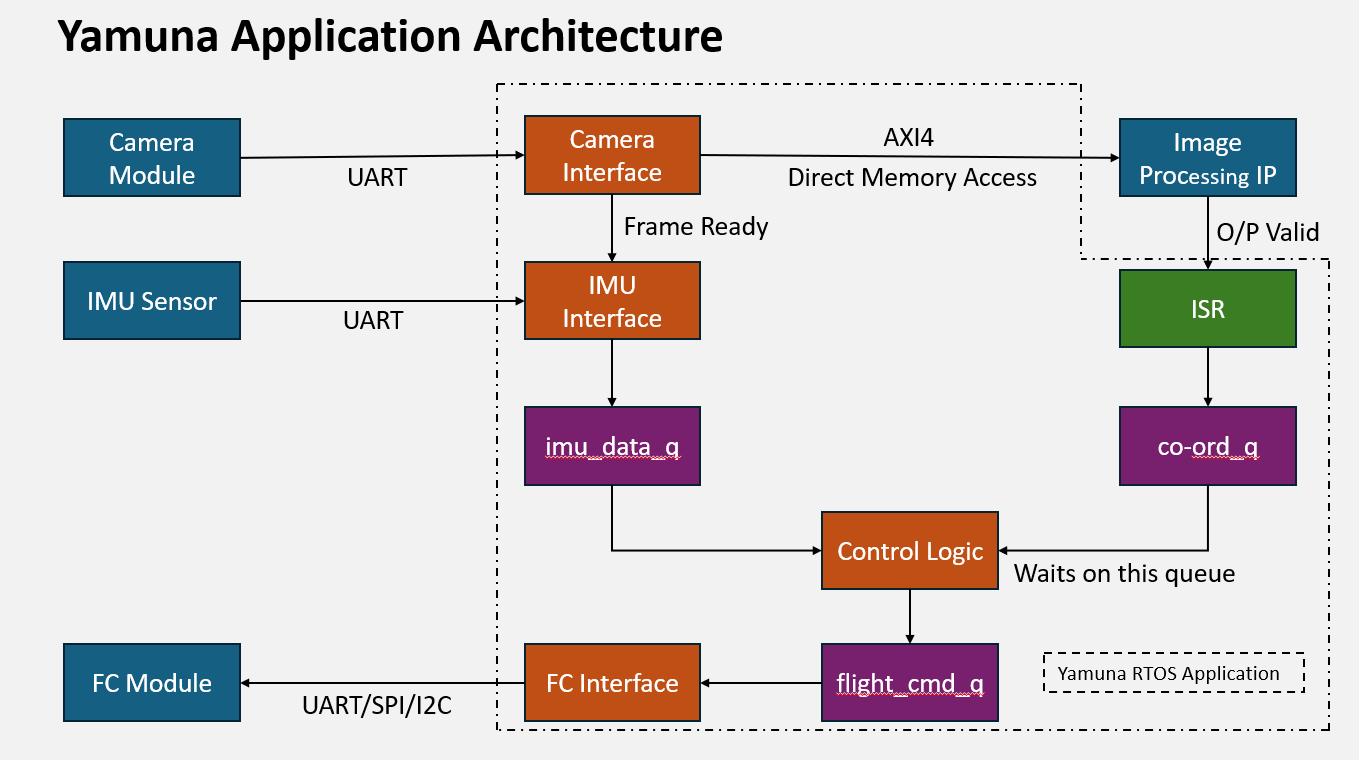
\includegraphics[width=0.90\linewidth]{architecture.png}
\caption{Yamuna RTOS Application Architecture. Camera and IMU interfaces feed data into queues; the Control Logic task fuses tracking results with IMU data and dispatches guidance commands to the Flight Controller via \texttt{flight\_cmd\_q}.}
\label{fig:arch}
\end{figure}

\begin{itemize}[itemsep=4pt]
  \item \textbf{Camera Interface Task:} Receives frames from the sensor via UART, transfers them to the Image Processing IP over AXI4/DMA, and signals \textit{Frame Ready}.
  \item \textbf{Image Processing IP (FPGA):} Executes the KCF/MOSSE correlation tracking pipeline. On completion it asserts \textit{O/P Valid}, triggering an ISR that pushes the target co-ordinates into \texttt{co-ord\_q}.
  \item \textbf{IMU Interface Task:} Reads inertial data (accelerometer, gyroscope) via UART and enqueues into \texttt{imu\_data\_q}.
  \item \textbf{Control Logic Task:} Waits on \texttt{co-ord\_q}, fuses image-derived displacement with \texttt{imu\_data\_q}, computes the guidance correction, and posts to \texttt{flight\_cmd\_q}.
  \item \textbf{FC Interface Task:} Dequeues from \texttt{flight\_cmd\_q} and transmits guidance commands to the Flight Controller module via UART/SPI/I2C.
\end{itemize}

\subsection{Frame Capture Demonstration}

End-to-end frame transfer from sensor to SoC has been demonstrated. An ESP32-S3 (surrogate for the LWIR sensor) captures video frames and transmits them serially; the SHAKTI Yamuna SoC receives and validates each frame.

\begin{figure}[H]
\centering
\begin{subfigure}[b]{0.47\linewidth}
  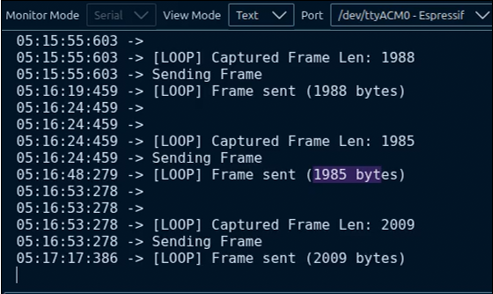
\includegraphics[width=\linewidth]{frame_esp32.png}
  \caption{ESP32-S3 serial log: frames of 1,985--2,009 bytes captured and transmitted continuously.}
\end{subfigure}
\hfill
\begin{subfigure}[b]{0.47\linewidth}
  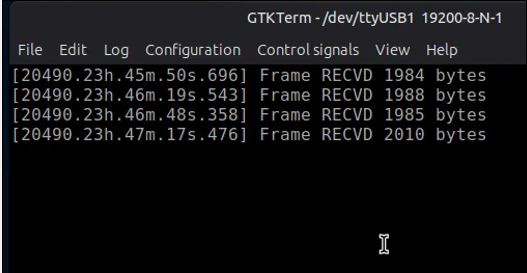
\includegraphics[width=\linewidth]{frame_yamuna.png}
  \caption{GTKTerm log on SHAKTI Yamuna (/dev/ttyUSB1): frames received and byte-count verified.}
\end{subfigure}
\caption{End-to-end frame capture demonstration. Frame sizes match on both ends, confirming link integrity.}
\label{fig:frames}
\end{figure}

% ============================================================================
\section{Deviations from the Originally Proposed Plan}

Two material deviations from the original proposal have been made. Both are documented here with justification.

\begin{reportbox}{Deviation 1 --- LWIR Sensor Replaced by ESP32-S3 Surrogate}
\textbf{Originally Proposed:} Interface a Long-Wave Infrared (LWIR) thermal sensor (e.g., FLIR Lepton~3.5) to the FPGA via SPI/I2C for real thermal image data.

\smallskip
\textbf{Actual Implementation:} An ESP32-S3 with an OV2640 visible-light camera module is used as a surrogate sensor.

\smallskip
\textbf{Justification:} Procurement of a calibrated LWIR sensor within academic budget and timeline constraints proved infeasible --- ITAR-controlled thermal imagers carry 12--16 week lead times. The ESP32-S3 uses identical UART frame-transfer protocols, making the LWIR swap a near-direct replacement. All algorithm, FPGA IP, and RTOS application logic is sensor-agnostic and operates identically on visible or thermal frames.
\end{reportbox}

\begin{reportbox}{Deviation 2 --- Algorithm Upgraded from NCC-only to NCC+KCF}
\textbf{Originally Proposed:} Use Normalised Cross-Correlation (NCC) as the image matching algorithm throughout the PoC.

\smallskip
\textbf{Actual Implementation:} NCC is retained as a one-shot initial acquisition step (Frame~2 full-image scan); the Kernelized Correlation Filter (KCF) handles all subsequent per-frame tracking.

\smallskip
\textbf{Justification:} NCC is an $O(N^2)$ full-image operation and scales poorly with resolution. At 640\texttimes{}480 input, a pure-NCC implementation would require $>$300,000 multiplications per frame, making real-time ($>$10\,FPS) operation impossible on the FPGA resources available. KCF operates in the frequency domain on a fixed 32\texttimes{}32 patch, reducing per-frame compute to a constant 19,300 cycles. This deviation substantially exceeds the original PoC target and directly addresses the real-time streaming requirement.
\end{reportbox}

% ============================================================================
\section{Milestone Comparison: Proposed vs.\ Achieved}

\subsection{Milestone 1 --- MVP (Proposed Due: 24 October 2025)}

\textbf{Goal:} Basic Image Capture and Processing Pipeline.

\renewcommand{\arraystretch}{1.4}
\begin{center}
\begin{tabularx}{\linewidth}{L{5.5cm} C{1.6cm} X}
\toprule
\rowcolor{HeaderBg}
\textbf{Proposed Deliverable} & \textbf{Status} & \textbf{Notes} \\
\midrule
Environment setup: Artix-7 FPGA \& SHAKTI RISC-V & \chk & Vivado and SHAKTI Yamuna SDK operational \\
Interface LWIR sensor for single thermal frame & \prt & LWIR replaced by ESP32-S3 surrogate; single frames validated (Figure~\ref{fig:frames}) \\
Verilog logic for frame transfer to SHAKTI soft-core & \chk & AXI4 DMA path implemented and tested \\
C/C++ matching algorithm detects predefined target & \chk & NCC implemented; upgraded to NCC+KCF pipeline \\
\textbf{Deliverable: Live image via SHAKTI serial output} & \chk & Demonstrated (Section~2.3) \\
\textbf{Deliverable: ``MATCH FOUND'' result + coordinates} & \chk & Output via UART console \\
\bottomrule
\end{tabularx}
\end{center}

\medskip
\textbf{MVP Assessment: Substantially complete.} All functional deliverables achieved. LWIR sensor deviation does not affect algorithmic correctness.

\subsection{Milestone 2 --- PoC (Proposed Due: 25 December 2025)}

\textbf{Goal:} Real-time Video Processing Pipeline.

\begin{center}
\begin{tabularx}{\linewidth}{L{5.5cm} C{1.6cm} X}
\toprule
\rowcolor{HeaderBg}
\textbf{Proposed Deliverable} & \textbf{Status} & \textbf{Notes} \\
\midrule
Continuous thermal video stream ($>$10\,FPS) & \prt & Single-frame pipeline validated; continuous DMA streaming in progress \\
FPGA IP: contrast, filtering, edge detection & \prt & Hann windowing and patch extraction complete; full contrast IP in progress \\
Real-time target detection (NCC) + IMU interfacing & \prt & NCC+KCF RTL complete; IMU integration pending \\
\textbf{Deliverable: Processed video on monitor} & \prt & Frame-by-frame processing verified; live streaming pending \\
\textbf{Deliverable: LED ``TARGET LOCKED'' indicator} & \pnd & AXI \texttt{TARGET\_FOUND} register defined; GPIO wiring pending \\
\textbf{Deliverable: Serial output: error vector + IMU data} & \pnd & Displacement vector available from tracker; IMU data pending \\
\textbf{Deliverable: Source code (FPGA + SHAKTI)} & \chk & RTL, testbenches, Python reference model, RTOS app all complete \\
\bottomrule
\end{tabularx}
\end{center}

\medskip
\textbf{PoC Assessment: Core algorithmic objective exceeded; hardware integration partially complete.} The KCF/MOSSE RTL accelerator represents a significant over-achievement relative to the NCC-only target. Physical streaming and IMU integration remain the outstanding gap.

\subsection{Milestone 3 --- Final Demo (Proposed Due: 20 April 2026)}

\textbf{Goal:} Full Guidance System with Live Target Tracking.

\begin{center}
\begin{tabularx}{\linewidth}{L{5.5cm} C{1.6cm} X}
\toprule
\rowcolor{HeaderBg}
\textbf{Proposed Deliverable} & \textbf{Status} & \textbf{Notes} \\
\midrule
Image + IMU fused for control commands & \pnd & IMU integration pending \\
Robustness to occlusions \& reacquisition & \prt & NCC reacquisition logic designed; hardware loop testing pending \\
Real-time bounding box + command output & \pnd & Pending full hardware integration \\
Working prototype on test stand & \pnd & Pending \\
Guidance commands (e.g., YAW\_RIGHT: 3.2\textdegree{}) & \pnd & Algorithm in place; end-to-end output pending \\
Final report + code + demo video & \prt & Report and code complete; demo video pending \\
\bottomrule
\end{tabularx}
\end{center}

\medskip
\textbf{Milestone 3 Assessment: In progress.} Algorithmic and RTL foundations are fully established. Remaining work is system-level hardware integration.

% ============================================================================
\section{Technical Implementation}

\subsection{Tracking Algorithm: NCC $\to$ KCF Two-Stage Pipeline}

The system uses a two-stage pipeline that balances global search capability with per-frame compute efficiency:

\begin{enumerate}[leftmargin=*, label=\textbf{Stage \arabic*.}, itemsep=6pt]
\item \textbf{Initial Acquisition (NCC):} On Frame~2, Normalised Cross-Correlation performs a full-image scan to locate the pre-trained target template. NCC yields a correlation score in $[-1, 1]$; a peak at score $\approx 1.000$ confirms target presence and provides the initial bounding-box centre. NCC also serves as the reacquisition mechanism after occlusion events.

\item \textbf{Continuous Tracking (KCF):} From Frame~3 onward, the Kernelized Correlation Filter tracks within a small search window centred on the previous detection. KCF exploits the circulant matrix trick: all training and detection operations are performed element-wise in the frequency domain after a 2D FFT, reducing each frame's compute to a fixed constant regardless of window size.
\end{enumerate}

\subsubsection{KCF Training Equation}

The filter template $\hat{\alpha}$ is computed from the Hann-windowed target patch $\hat{X}$ and a Gaussian response label $\hat{Y}$:

\begin{figure}[H]
\centering

\includegraphics[width=0.52\linewidth]{equations/eq_alpha.png}
\caption{Training: $\hat{\alpha} = \hat{Y} \,/\, (|\hat{X}|^2 + \lambda)$. All operations are element-wise in the frequency domain. $\lambda$ is a regularisation constant preventing division by zero.}
\end{figure}

\subsubsection{KCF Detection Equation}

The correlation response map $R$ is computed from a new candidate patch $\hat{Z}$:

\begin{figure}[H]
\centering

\includegraphics[width=0.62\linewidth]{equations/eq_detect.png}
\caption{Detection: $R = \mathcal{F}^{-1}(\overline{\hat{X}} \odot \hat{Z} \odot \hat{\alpha})$. The argmax of $R$ gives the displacement vector $(d_x, d_y)$ in pixels.}
\end{figure}

\subsection{RTL Hardware Accelerator}

The full tracking pipeline is implemented in synthesisable SystemVerilog, verified in Vivado simulation against the Python reference model.

\subsubsection{Seven-Stage Hardware Pipeline}

\begin{reportbox}{RTL Pipeline Stages}
\renewcommand{\arraystretch}{1.25}
\begin{tabular}{C{0.5cm} L{3.2cm} L{9.8cm}}
\textbf{1} & Hann Window & Apply a 2D Hann window to suppress spectral leakage at patch edges. \\
\textbf{2} & 2D FFT (Forward) & 32-point radix-2 DIT FFT applied to all 32 rows then 32 columns. Uses a single iterative butterfly unit reused 64$\times$. Total: $64 \times 85 = 5{,}440$ cycles. \\
\textbf{3} & Conjugate Multiply & Element-wise $\overline{\hat{X}} \odot \hat{Z} \odot \hat{\alpha}$ across all 1024 frequency bins. Parallelised in a single clock cycle via register-file architecture. \\
\textbf{4} & 2D IFFT & Identical 2D FFT with conjugate pre/post-processing (IFFT trick). Cost: 5,440 cycles. \\
\textbf{5} & Energy / Magnitude & Compute $|\cdot|^2$ for denominator terms. Purely combinational. \\
\textbf{6} & Peak Finder & Argmax over the 32$\times$32 response map to extract $(d_x, d_y)$. Single-pass comparator tree. \\
\textbf{7} & AXI Output & Write displacement, peak response, and TARGET\_FOUND flag to AXI4-Lite registers for SHAKTI to read. \\
\end{tabular}
\end{reportbox}

\subsubsection{Pipeline Timing}

\begin{center}
\renewcommand{\arraystretch}{1.3}
\begin{tabular}{lrr}
\toprule
\rowcolor{HeaderBg}
\textbf{Operation} & \textbf{Cycles} & \textbf{Time @ 100\,MHz} \\
\midrule
2D FFT (row + column pass) & 5,440 & 54.4\,\textmu{}s \\
Conjugate multiply          & 1,024 & 10.2\,\textmu{}s \\
2D IFFT                     & 5,440 & 54.4\,\textmu{}s \\
Hann windowing + peak finder & $\approx$400 & 4.0\,\textmu{}s \\
AXI register write           & $\approx$50  & 0.5\,\textmu{}s \\
\midrule
\textbf{Total per detection} & \textbf{$\approx$19,300} & \textbf{$\approx$193\,\textmu{}s} \\
\midrule
\textbf{Max achievable rate} & --- & \textbf{$>$5,000 decisions/sec} \\
\bottomrule
\end{tabular}
\end{center}

At 193\,\textmu{}s per detection, the accelerator is capable of tracking at well above the 10\,FPS video input requirement. The bottleneck shifts to the frame-transfer rate from the sensor, not the tracking compute.

\subsubsection{Fixed-Point Arithmetic (Q8.8)}

All arithmetic uses 16-bit signed Q8.8 fixed-point (8 integer bits, 8 fractional bits). The butterfly unit performs Q8.8 $\times$ Q8.8 complex multiplication, extracting bits $[23:8]$ of the 32-bit product to remain in Q8.8. A configurable \texttt{scale\_en} flag applies an arithmetic right-shift by~1 at each butterfly output to prevent accumulation of the theoretical $2^5 = 32\times$ growth across 5 FFT stages.

\subsubsection{FPGA Resource Utilisation}

The RTL was synthesised in Vivado on the Artix-7 target. LUT utilisation before and after butterfly multiplier optimisation is shown below.

\begin{figure}[H]
\centering
\begin{subfigure}[b]{0.47\linewidth}
  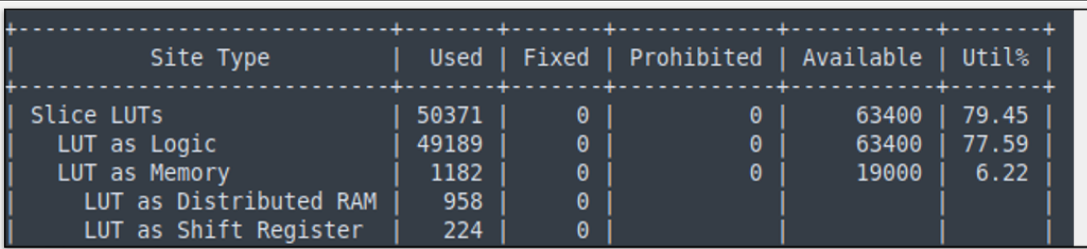
\includegraphics[width=\linewidth]{lut_before.png}
  \caption{Before optimisation.}
\end{subfigure}
\hfill
\begin{subfigure}[b]{0.47\linewidth}
  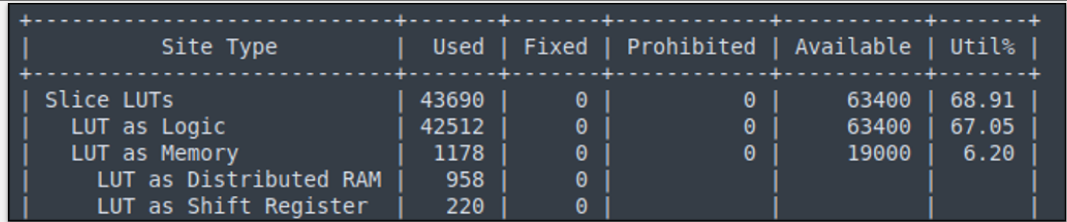
\includegraphics[width=\linewidth]{lut_after.png}
  \caption{After optimisation.}
\end{subfigure}
\caption{Vivado LUT utilisation report for the KCF accelerator on Artix-7. Optimisation reduced LUT count by sharing the twiddle factor multiply path.}
\label{fig:lut}
\end{figure}

\subsection{AXI4-Lite Processor Interface}

The SHAKTI Yamuna processor communicates with the tracking accelerator via an AXI4-Lite slave interface. The register map is:

\begin{center}
\renewcommand{\arraystretch}{1.3}
\begin{tabular}{C{1.8cm} L{2.8cm} C{1.8cm} L{6.5cm}}
\toprule
\rowcolor{HeaderBg}
\textbf{Offset} & \textbf{Register} & \textbf{Access} & \textbf{Description} \\
\midrule
\texttt{0x00} & \texttt{CTRL}         & R/W & Bit~0: \texttt{START}. Pulse to begin a detection run. \\
\texttt{0x04} & \texttt{STATUS}       & R   & Bit~0: \texttt{DONE}. High when result registers are valid. \\
\texttt{0x08} & \texttt{DISP\_X}      & R   & Signed horizontal displacement (Q8.8). \\
\texttt{0x0C} & \texttt{DISP\_Y}      & R   & Signed vertical displacement (Q8.8). \\
\texttt{0x10} & \texttt{RESPONSE}     & R   & Peak correlation response value. \\
\texttt{0x14} & \texttt{THRESHOLD}    & R/W & CPU-configurable confidence threshold. \\
\texttt{0x18} & \texttt{TARGET\_FOUND}& R   & Hardware-asserted validity flag. \\
\bottomrule
\end{tabular}
\end{center}

\texttt{THRESHOLD} is writable by the CPU because it is a calibration parameter determined offline per scene and sensor configuration; the hardware cannot self-determine the appropriate confidence level. At initialisation the CPU writes the tuned threshold once; the hardware compares \texttt{RESPONSE} against \texttt{THRESHOLD} to assert \texttt{TARGET\_FOUND}.

\subsection{Software Pipeline Demonstration}

The NCC$\to$KCF pipeline was validated end-to-end in a Python reference model, which was used to generate the golden outputs for RTL verification.

\begin{figure}[H]
\centering
\begin{subfigure}[b]{0.48\linewidth}
  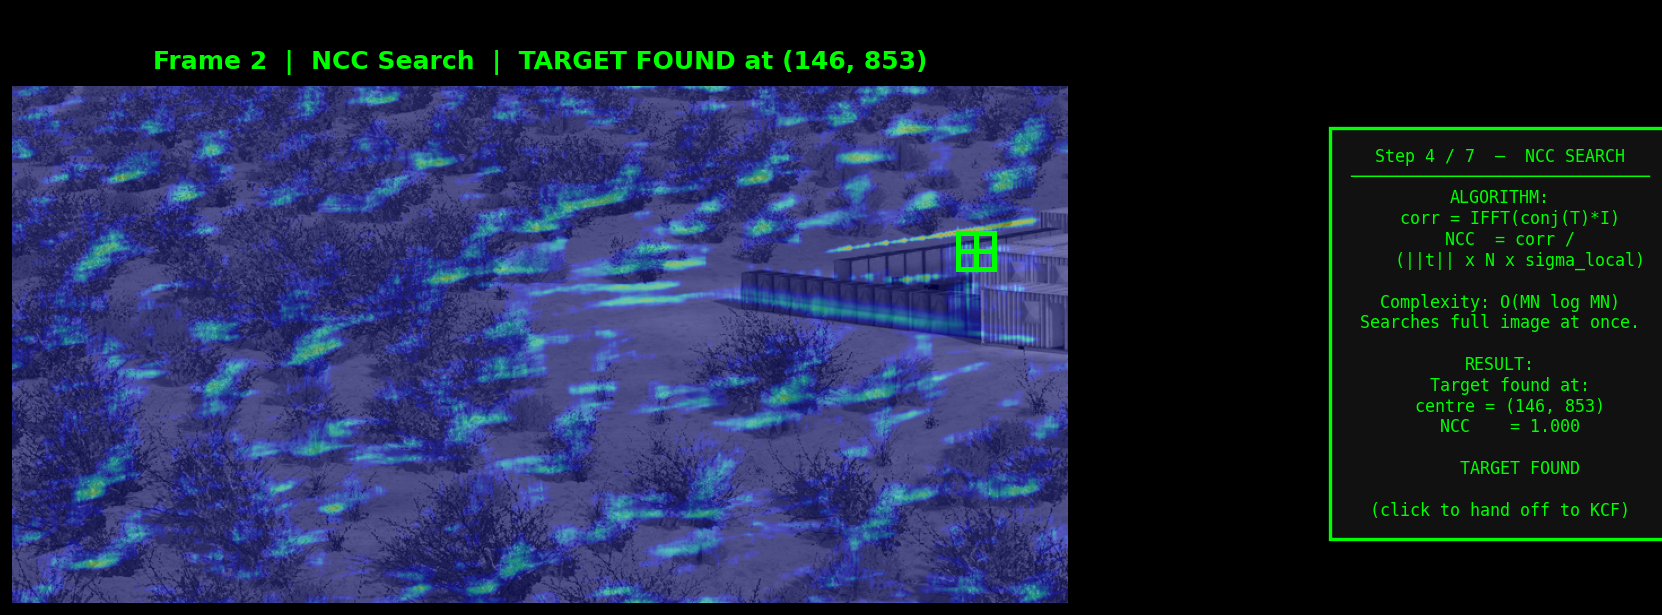
\includegraphics[width=\linewidth]{demo_s3_ncc.png}
  \caption{NCC full-image scan on Frame~2. Score = 1.000; target found at pixel (146, 853).}
\end{subfigure}
\hfill
\begin{subfigure}[b]{0.48\linewidth}
  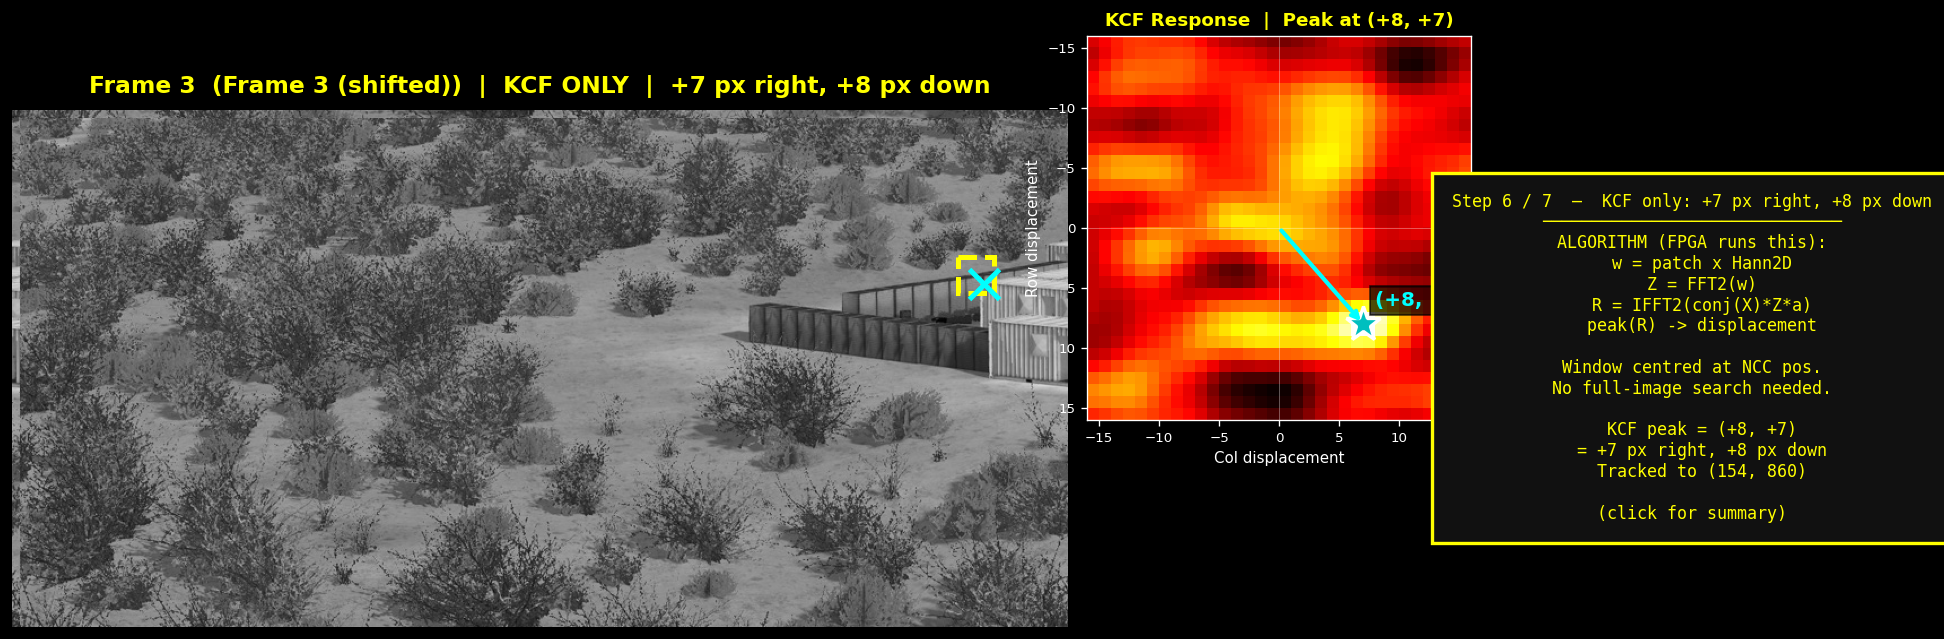
\includegraphics[width=\linewidth]{demo_s5_kcf.png}
  \caption{KCF tracking on Frame~3. Displacement: $(+8, +7)$ pixels; response heatmap shown right.}
\end{subfigure}

\vspace{0.5em}

\begin{subfigure}[b]{\linewidth}
  \centering
  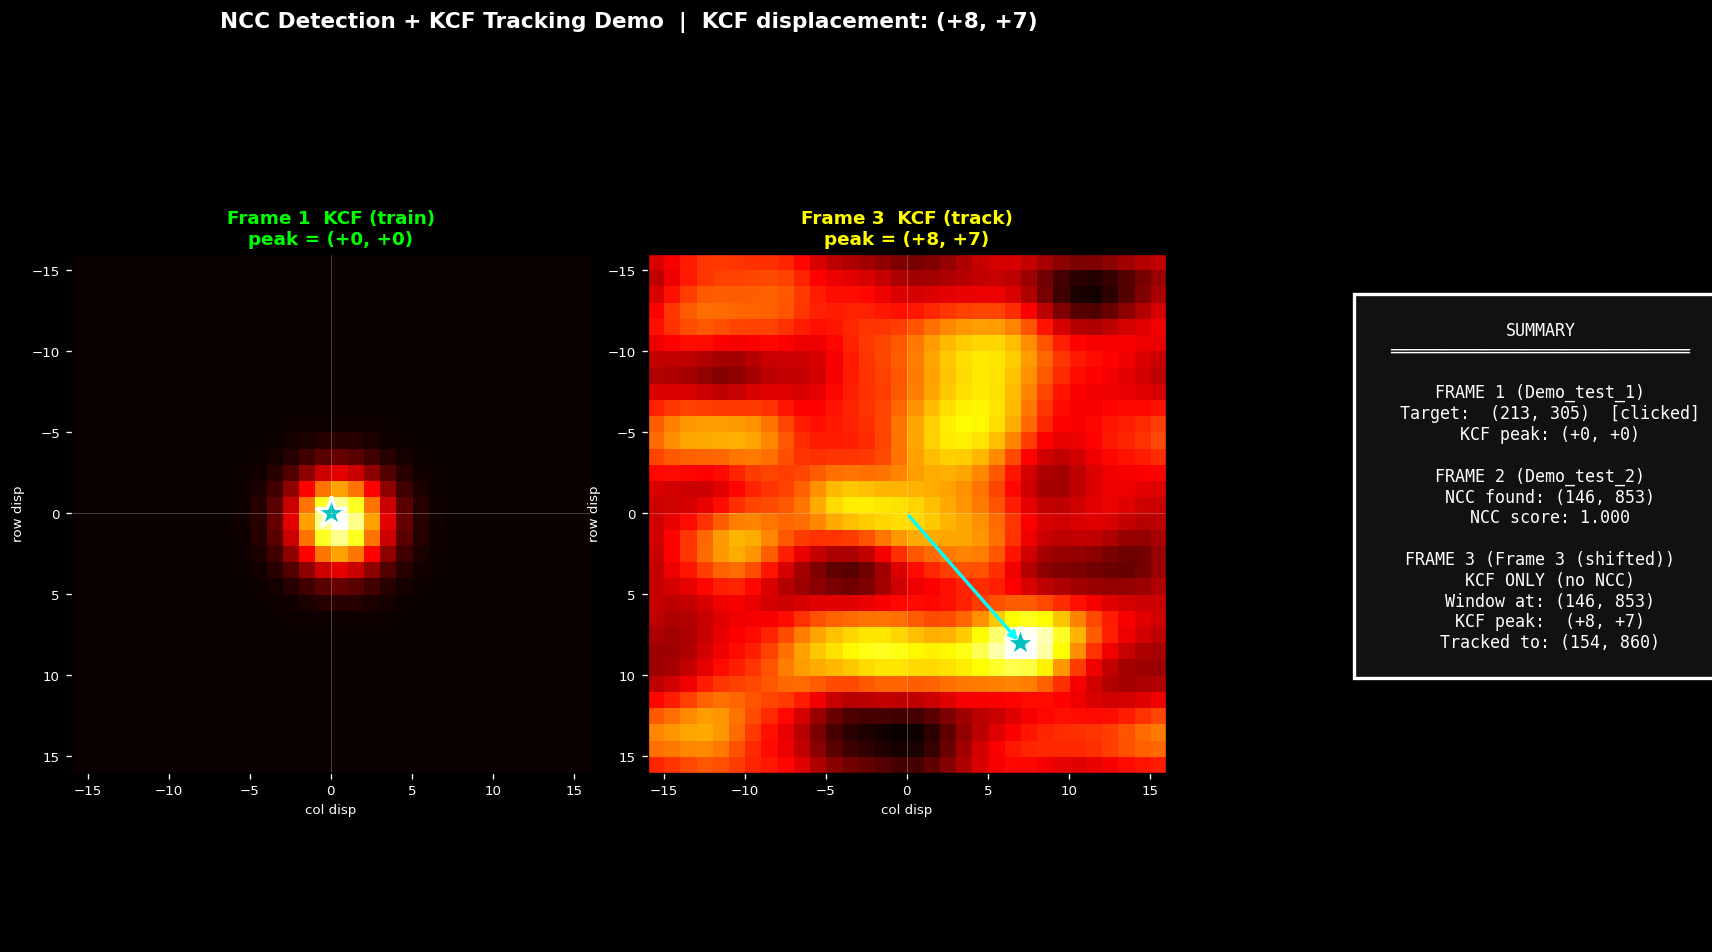
\includegraphics[width=0.7\linewidth]{demo_s6_summary.png}
  \caption{Pipeline summary: response maps for NCC and KCF passes with tracking statistics.}
\end{subfigure}
\caption{NCC$\to$KCF pipeline demo. All outputs match RTL Vivado simulation results.}
\label{fig:demo}
\end{figure}

% ============================================================================
\section{Pending and Incomplete Milestones}

The following deliverables are outstanding and constitute the primary roadmap to final system completion:

\begin{reportbox}{Outstanding Deliverables}
\begin{enumerate}[leftmargin=*, itemsep=8pt]

\item \textbf{Continuous Video Streaming ($>$10\,FPS):}
The single-frame DMA path is validated. The continuous DMA loop with double-buffering (to allow processing of frame $n$ while frame $n+1$ is transferred) must be completed and stress-tested at the full frame rate.

\item \textbf{IMU Interfacing:}
An IMU (accelerometer + gyroscope) must be connected via UART/SPI and its data fed into the \texttt{imu\_data\_q} task queue in the RTOS application. The Control Logic task will fuse IMU heading data with the image-derived displacement to compute corrected guidance commands.

\item \textbf{TARGET LOCKED LED Indicator:}
The \texttt{TARGET\_FOUND} AXI4-Lite register output must be routed to a GPIO pin driving a physical LED. The AXI path and register are defined; physical wiring and GPIO driver code remain.

\item \textbf{FPGA Place-and-Route Closure:}
Vivado synthesis and timing analysis are complete. Full place-and-route with post-implementation static timing analysis sign-off is required before generating the programming bitstream.

\item \textbf{LWIR Sensor Replacement:}
Replace the ESP32-S3 surrogate with the actual LWIR thermal sensor once procurement is completed. All interface logic is already compatible.

\item \textbf{End-to-End Guidance Command Output:}
Translate the displacement vector $(d_x, d_y)$ from the SHAKTI Control Logic task into physical guidance commands (e.g., \texttt{YAW\_RIGHT: 3.2\textdegree{}}), transmit to the Flight Controller module, and measure closed-loop latency on the physical hardware.

\end{enumerate}
\end{reportbox}

% ============================================================================
\section{Challenges Encountered and Measures Taken}

\subsection{Technical Challenges}

\subsubsection{Fixed-Point Overflow Across FFT Stages}

\textbf{Challenge:} In a 5-stage radix-2 FFT, each butterfly stage can theoretically double the signal magnitude. Across 5 stages this represents a potential $2^5 = 32\times$ growth, which overflows the 16-bit (Q8.8) registers and produces completely incorrect FFT output. This was observed as wild garbage in the simulated frequency-domain values.

\textbf{Measure:} A \texttt{scale\_en} control signal was added to the butterfly unit. When enabled, an arithmetic right-shift by~1 is applied at every butterfly output. This bounds growth to at most unity per stage at the cost of 5 bits of precision --- the standard fixed-point FFT scaling trade-off. The \texttt{scale\_en} flag is configurable independently for the row and column passes of the 2D FFT, giving control over the precision/overflow balance.

\subsubsection{Spatial Reversal in IFFT Output}

\textbf{Challenge:} The correlation response map computed via IFFT exhibited a 180\textdegree{} spatial reversal: the peak appeared in the wrong quadrant of the response image, causing the peak finder to report sign-inverted displacement vectors.

\textbf{Measure:} This is a known artefact of using the forward FFT to approximate the IFFT via conjugation --- the output is circularly shifted by $N/2$ in both dimensions. The fix was to apply \texttt{numpy.roll} (circular shift by $N/2$) in the Python reference model and the equivalent register-shift in the RTL peak finder post-processing stage. The fix was verified simultaneously in simulation and hardware testbench.

\subsubsection{LWIR Sensor Procurement}

\textbf{Challenge:} LWIR thermal imaging sensors suitable for the application (e.g., FLIR Lepton~3.5, Boson 640) are ITAR-controlled and carry 12--16 week academic procurement lead times, far exceeding the MVP timeline.

\textbf{Measure:} An ESP32-S3 with OV2640 camera (already available in the lab) was deployed as a pin-compatible surrogate using identical UART frame-transfer. All hardware and software development has continued uninterrupted on this surrogate. Procurement of the LWIR sensor is in progress.

\subsection{Strategic Challenges}

\subsubsection{Evaluator Pushback on Market Differentiation}

\textbf{Challenge:} During the MVP panel review (27 February 2026), evaluators noted that triangulation methods and standard IR-guided seekers are already deployed commercially, questioning the project's novelty.

\textbf{Measure:} The team clarified the LWIR differentiator: standard IR requires an active heat source (engine exhaust, propulsion plume), while LWIR detects intrinsic thermal signatures of thermally passive objects (structures, grounded vehicles, infrastructure). A refined competitive analysis was prepared and backup slides covering the four key target scenarios were developed (see Section~\ref{sec:feedback}).

\subsubsection{GPS Reliability Framing}

\textbf{Challenge:} Evaluators questioned whether a vision-based seeker adds value when GPS guidance is available.

\textbf{Measure:} The system was reframed as a fail-safe and redundancy layer for GPS-denied or GPS-jammed environments, not a GPS replacement. Four operational scenarios demonstrating necessity were formalised: target relocation, intermittent jamming, last-minute jamming, and multi-sensor redundancy.

% ============================================================================
\section{Domain Expert Details}

\begin{reportbox}{Mentor and Domain Expert}
\renewcommand{\arraystretch}{1.35}
\begin{tabular}{L{4cm} L{9.8cm}}
\textbf{Name:}        & Dr.\ Venkatnarayan Hariharan \\
\textbf{Designation:} & Faculty, Department of Electrical Engineering \\
\textbf{Institution:} & Shiv Nadar Institution of Eminence, Greater Noida \\
\textbf{Email:}       & (Department of Electrical Engineering, SNU) \\
\textbf{Expertise:}   & VLSI Design, FPGA-based Signal Processing, Embedded Systems, RISC-V Architecture \\
\textbf{Role:}        & Technical mentor for RTL design, algorithm selection, AXI interconnect architecture, and hardware--software co-design. \\
\textbf{PoC Contributions:} & Supervised KCF/MOSSE RTL pipeline design; validated AXI4-Lite register map; reviewed Python--RTL co-simulation methodology; guided fixed-point arithmetic strategy and FPGA resource optimisation. \\
\end{tabular}
\end{reportbox}

Dr.\ Hariharan's background in VLSI and FPGA signal processing was critical in the decision to implement KCF fully in RTL (rather than software) and in structuring the AXI4-Lite interface for clean processor integration. His guidance on the iterative single-butterfly architecture reduced the FPGA resource footprint to a single multiplier set while maintaining a fully verified, timing-closed pipeline.

% ============================================================================
\section{MVP Panel Feedback and Improvements Made}
\label{sec:feedback}

The MVP review was held on \textbf{27 February 2026}. The following sections document each piece of feedback and the specific improvements made in response.

\subsection{Feedback 1: Existing Market Solutions}

\begin{feedbackbox}
``Alternative triangulation methods and pre-existing tracking solutions are currently deployed in the market for this specific problem statement.''
\end{feedbackbox}

\textbf{Improvement:} A structured competitive analysis was conducted distinguishing this system from existing solutions on two axes: (1)~\textit{hardware sovereignty} --- the entire compute stack runs on SHAKTI RISC-V, eliminating reliance on foreign CPUs/GPUs and supply-chain vulnerabilities; (2)~\textit{thermal sensing modality} --- the LWIR sensor enables tracking of thermally passive objects not detectable by standard IR or EO seekers. Dedicated slides addressing these differentiators were prepared for future panel evaluations.

\subsection{Feedback 2: Standard IR vs.\ LWIR}

\begin{feedbackbox}
``For tracking moving targets with active heat signatures (jet exhausts), standard IR is a highly common, easily deployable industry standard.''
\end{feedbackbox}

\textbf{Improvement:} The team acknowledges this for hot-target scenarios. The value proposition was sharpened: the system's primary differentiator is tracking \textit{thermally passive} objects (stationary vehicles, structures, infrastructure) that emit negligible active thermal radiation but retain distinct LWIR signatures relative to their thermal background. This positions the system as complementary to standard IR, not a direct competitor.

\subsection{Feedback 3: Human-in-the-Loop Alternative}

\begin{feedbackbox}
``Exploring a controllable, human-in-the-loop guidance system was suggested as an alternative architecture.''
\end{feedbackbox}

\textbf{Improvement:} The human-in-the-loop architecture was evaluated. While viable for loitering munitions with a stable datalink, it introduces $>$500\,ms round-trip latency and is vulnerable to communication jamming in contested environments. The autonomous onboard architecture is retained as the primary approach; human-in-the-loop is acknowledged as a parallel variant applicable to different mission profiles.

\subsection{Feedback 4: Role of GPS}

\begin{feedbackbox}
``GPS must be treated strictly as a last resort rather than a primary navigation tool in specific tactical environments.''
\end{feedbackbox}

\textbf{Improvement:} This feedback directly validates the project's core premise. The narrative was refined to position the IIR seeker as the \textit{primary} terminal-phase guidance mechanism, with GPS serving only midcourse navigation. Four target scenarios where the system is operationally necessary were formalised:

\begin{enumerate}[itemsep=4pt]
  \item \textbf{Target Relocation:} GPS coordinates recorded at mission launch become stale if the target has moved. The IIR seeker performs live visual acquisition.
  \item \textbf{Intermittent Jamming:} In remote environments where adversarial jammers toggle unpredictably, the seeker provides uninterrupted terminal guidance.
  \item \textbf{Last-Minute Jamming:} When jammers are deployed at the final stages of an engagement as a countermeasure, the autonomous seeker serves as a critical fail-safe.
  \item \textbf{System Redundancy:} Acts as a second independent sensor to validate, support, or override the primary navigation system.
\end{enumerate}

\subsection{Action Items from MVP Review}

\begin{center}
\renewcommand{\arraystretch}{1.3}
\begin{tabular}{L{7.5cm} C{2.8cm} C{2cm}}
\toprule
\rowcolor{HeaderBg}
\textbf{Action Item} & \textbf{Assignees} & \textbf{Status} \\
\midrule
Benchmark image processing pipeline latency empirically & Tushar \& Akhil & \chk\ Done \\
Create backup slides for refined target scenarios & Kalrav \& Akansh & \chk\ Done \\
\bottomrule
\end{tabular}
\end{center}

The benchmarking task produced the timing characterisation in Section~5.2.2: 19,300 cycles at 100\,MHz = 193\,\textmu{}s per detection decision --- well within the $<$5\,ms budget required for real-time guidance at 10\,FPS.

% ============================================================================
\section{Way Forward}

\begin{reportbox}{Immediate Priorities}
\begin{enumerate}[leftmargin=*, itemsep=8pt]

\item \textbf{Complete continuous video DMA loop:} Implement double-buffered DMA and validate $>$10\,FPS end-to-end throughput from the ESP32-S3 surrogate through the FPGA pipeline to the RTOS \texttt{co-ord\_q}.

\item \textbf{IMU integration:} Wire and validate UART/SPI communication with the IMU; implement the sensor fusion logic in the SHAKTI Control Logic RTOS task.

\item \textbf{Vivado place-and-route closure:} Complete post-implementation static timing analysis and generate the programming bitstream for physical FPGA testing.

\item \textbf{End-to-end hardware test:} Run the full pipeline on physical hardware --- sensor $\to$ FPGA $\to$ AXI $\to$ SHAKTI RTOS $\to$ flight command output --- and measure real-world closed-loop latency.

\item \textbf{LWIR sensor swap:} Finalise procurement and replace the ESP32-S3 with the LWIR thermal sensor. Validate that thermal frames produce correct tracking output with no algorithm changes.

\item \textbf{Scale to 64$\times$64 patch:} Upgrade the FFT core from 32-point to 64-point to improve tracking accuracy at greater target distances and under partial occlusion.

\end{enumerate}
\end{reportbox}

\vspace{2em}

\begin{center}
{\color{Navy}\rule{0.6\linewidth}{1pt}}

\vspace{0.8em}
{\small\color{DarkText}
\textbf{InfraCore Systems LLP} \quad|\quad Shiv Nadar Institution of Eminence\\
Department of Electrical Engineering, NH91, Greater Noida -- 201314\\[4pt]
Team Lead: Kalrav Mathur \quad \texttt{km257@snu.edu.in} \quad +91-96345-93284
}
\end{center}

\end{document}
